\chapter{The Line}
\label{ch:29}



\begin{center}
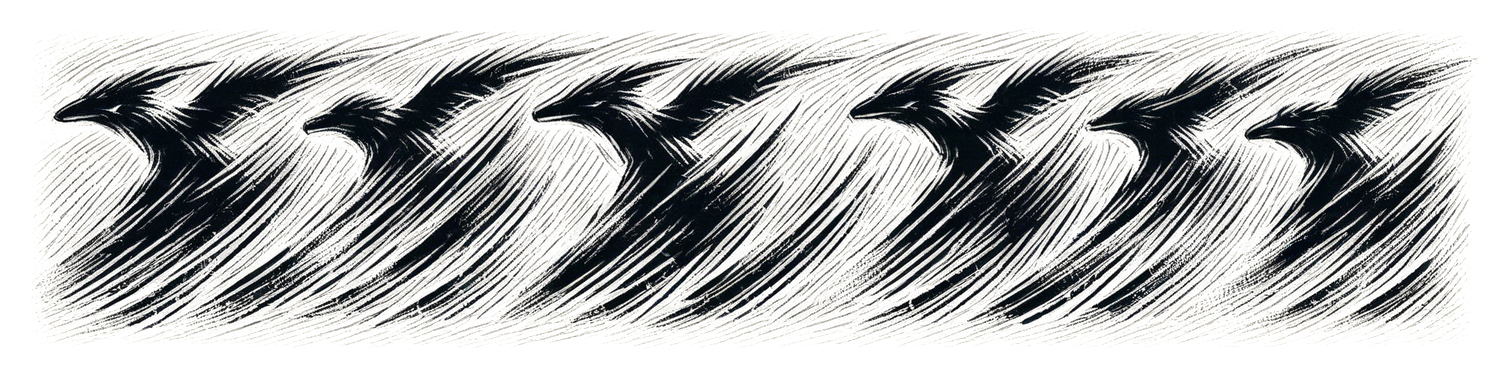
\includegraphics[width=\textwidth]{images/chapterImages/genesis_sketch_00126_.png}
\end{center}

The calibration locked in at 23:47. Sixteen months of work. Done.

The hum in Sarah's head—the constant pressure that had pushed her through meals, through sleep, through Maya's graduation last year—went quiet.

The silence was worse.

Marcus was staring at the screen. She watched his shoulders drop. He felt it too.

"That's it," he said.

She didn't answer.

They'd been alone at the site for six days. The rest of the team rotated out. Someone had to stay. Monitor. Verify. They both volunteered. Of course they did. The compulsion demanded it.

Except now the compulsion was gone. This section was complete.

Marcus turned. His face was wrong—too open, too raw. Like skin that had been bandaged for years suddenly exposed.

"I don't know what to do now," he said.

Sarah's hands were shaking. When had they started shaking?

"Yeah."

He stood. Crossed the room. Stopped three feet away.

The space between them felt like pressure. Like the absence of the compulsion had created a vacuum.

"I can't tell—" he started, then stopped.

"What?"

"If I want this or if I just need something to fill the fucking quiet."

Sarah looked at him. Really looked. Forty-three years old. Hadn't slept more than four hours straight in fifteen years. David's ring still on a chain under his shirt—she'd seen it once when he was reaching for tools overhead.

She didn't know what she felt. Couldn't separate it.

Exhaustion. Relief. Grief for her own losses. Attraction—when had that started? Or had it always been there, buried under the work?

Maybe it was just bodies recognizing each other. Two animals who'd survived the same thing.

"Come here," she said.

He hesitated.

"I don't know if—"

"Neither do I. Come here anyway."

He moved. She stood. His hand found her wrist. Her pulse hammering.

Was that him or the fifteen-year adrenaline crash?

Did it matter?

His mouth on hers. Desperate, not tender. Like drowning people gasping.

Her back against the console. His hands yanking at her shirt. No finesse. Just need.

She bit his lip. Tasted blood. He made a sound.

This wasn't soft. Wasn't meaningful. Was it?

Or was it the most meaningful thing she'd done in years because it was pointless, unnecessary, just for this moment, just because they were alive and the compulsion was quiet and nothing was making them do this?

Her nails dragged down his back. He pushed against her, hard enough to hurt.

Good. She wanted it to hurt. Wanted proof this was real, not programmed, not calculated.

Except how would she know?

The modified mammals—did they feel this? This confusion of want and need and choice and instinct?

Did Aurelia?

Marcus pulled back. Breathing hard.

"We should stop."

"Why?"

"I don't know if this is us or if it's—"

"Shut up."

She pulled him down. They went to the floor. Concrete cold against her spine. His weight on her. Real. Solid. Warm.

No grace to it. Fumbling with clothes. Too fast. Too rough.

She thought: this is animal.

Then: what else would it be?

Then: did Aurelia's mate pin her against prehistoric stone like this? Did she stop caring whether it meant something or if it was just cells following chemical commands?

Did she just... feel it?

Sarah stopped thinking.

\scenebreak

After.

Lying on the floor. Marcus's arm over his eyes. Her shirt half-on. Both breathing like they'd run.

The compulsion still quiet.

This new feeling in her chest—sharp, aching. What was it?

Regret? Satisfaction? Connection?

Grief?

She didn't know.

"David asked me once," Marcus said to the ceiling, "if I needed him or wanted him."

Sarah waited.

"I said I didn't know. He said that was the point. Said if I could tell the difference, it probably wasn't real."

Silence.

"Was he right?" Sarah asked.

"I still don't know."

She sat up. Found her pants. Dressed without looking at him.

"I think about her sometimes," she said. "Aurelia."

Marcus sat up too.

"Yeah."

"She had a mate. Young. She left them. Spent months calculating. When he died, she stopped for three days. Then went back to work."

"I know."

"Was that—" Sarah stopped. Started again. "Was she choosing the work over him? Or was the work... for him?"

Marcus was quiet for a long time.

"Maybe there's no difference," he said finally.

Sarah looked at the screen. The calibration still locked. Perfect. Complete.

All those years of compulsion. Building this. Sacrificing for it.

For what? The future. The planet. People not born yet.

For Maya. For David who died building it. For Aurelia who never saw it work.

The feeling in her chest sharpened.

"I don't know what this was," she said.

Marcus stood. Faced her.

"Me neither."

"Does it have to be something?"

"Doesn't everything?"

She almost laughed.

"The code made us able to build this," she gestured at the screen. "It didn't make us do... that."

"Didn't it?"

"I don't know. I can't tell anymore. What's programmed. What's choice. What's—"

She stopped.

Marcus finished: "What's real?"

"Yeah."

He pulled his shirt on. Turned to the window. Dawn coming.

"David said something else," he said. "The day he died. He said, 'I don't care if it's chemicals. I don't care if it's evolution. I choose you. Every day. That makes it real.'"

Sarah felt it again. That sharp thing in her chest.

Oh.

That's what it was.

Not the feeling itself—she still couldn't name it, couldn't separate it from biology and trauma and exhaustion.

But the choosing. The doing it anyway. Even uncertain. Even confused.

Aurelia chose to keep working after her mate died.

Not because she didn't feel something.

Because she felt it and worked anyway.

The feeling and the action. Both real. Both valid. Both... enough.

"We should run diagnostics," Sarah said.

Marcus looked at her. Something passed between them. Not understanding. Just... acknowledgment.

"Yeah."

They turned to the console.

The compulsion hummed back to life. Different section. More work.

Sarah didn't resent it.

It wasn't separate from what they'd just done. It was the same thing. The same confused tangle of instinct and choice and need and purpose.

She'd stopped trying to untangle it.

Maybe Aurelia had too.

\scenebreak

They worked through the morning in silence. The new section required attention. The compulsion had returned with familiar force. Relief and imprisonment simultaneously.

Sarah's body ached. The floor had been unforgiving. She had bruises forming where she'd hit the console edge. Her lip was split from where Marcus had pushed too hard.

She felt them all. Catalogued them. Proof that something had happened. Something real. Something that left marks.

At noon, Marcus made coffee. Brought her a cup. Set it down next to her workstation without speaking.

She drank it. Black, bitter, perfect.

They didn't talk about what had happened. Didn't need to. What would they say?

That was confusing?
That was desperate?
That was wrong?
That was right?
All of it true. None of it useful.

"System's stable," Marcus said eventually. "We could rotate out. Let the next team take over."

Sarah looked at the screen. At the work that still needed doing. At the thousand small adjustments and verifications that would take weeks.

"We could," she said.

Neither of them moved.

"I should call Maya," Sarah said. "Her graduation was eight months ago and I didn't even— I should call her."

"Will you?"

"Probably not."

"Yeah."

More silence. The equipment hummed. The mountain wind rattled something outside. The world continued.

"Did you feel it?" Sarah asked suddenly. "When the compulsion stopped? Did you feel... empty?"

Marcus considered this. "Not empty. Exposed. Like armor coming off. Like suddenly remembering I was human and not just a function."

"And then?"

"And then I didn't want to be human. Because being human hurts. Being a function is easier."

"But the compulsion came back."

"Yeah."

"Do you think it'll ever really stop?"

"I think this work will finish eventually. Decades maybe. And then—" He stopped.

"Then what? Next activation? Next threshold? We keep getting programmed for new purposes until we die?"

"Or until the program decides we're obsolete."

Sarah hadn't thought about that. What happened to tools that had served their function? Were they discarded? Repurposed? Or just left to break down naturally while new tools were activated?

"Maybe that's okay," she said. "Maybe having a purpose, even a programmed one, is better than meaningless existence."

"You trying to convince me or yourself?"

"Both."

Marcus smiled slightly. The first time she'd seen him smile in months. It transformed his face. Made him look younger. Almost happy.

Then the compulsion surged—a new problem needing attention—and the smile faded. He turned back to his screen.

Sarah watched him for a moment. This man she'd just fucked on a concrete floor. This man she barely knew beyond shared compulsion and shared loss. This man who understood without needing explanation.

Was that connection? Or just recognition?

Did the distinction matter?

Her hands moved over her keyboard. Adjusting parameters. Solving problems. Doing what the code demanded.

And underneath the work, the ache in her body. The split lip. The bruises forming.

Proof that she could still feel something that wasn't programmed.

Or was pain programmed too? Was everything?

She didn't know.

Kept working anyway.

\scenebreak

That evening, they ate together. Freeze-dried meals rehydrated with questionable water. Sitting at the small table in the facility's break room.

"Maya must be almost grown now," Marcus said.

Sarah looked up, surprised. "Nineteen. She's in college. Pre-med."

"You talk to her?"

"Christmas. Her birthday. Sometimes." Always brief. Always strained. Always ending with Maya's quiet disappointment and Sarah's defensive guilt.

"She knows about the compulsion?"

"She knows I chose work over her. Whether she understands the genetic component—" Sarah shrugged. "I don't know if she believes it. Or if she thinks it's an excuse."

"Is it an excuse?"

"I don't know. Does it matter?"

Marcus pushed food around his plate. "David's parents blame me. Say I could have fought it. Could have chosen him over the work. Maybe they're right."

"Or maybe they need someone to blame."

"Or maybe I'm a coward who used genetics as justification for abandoning someone I loved."

Sarah had no answer for that. She'd asked herself the same question about Maya ten thousand times.

"The woman who tried to resist," Marcus said after a long pause. "The engineer who went off-grid. You remember her?"

"Yeah."

"She said it was like trying not to breathe. Physical agony. Mental breakdown. Two weeks and she cracked."

"I remember."

"What if she'd lasted three weeks? A month? Would the compulsion have killed her?"

"I don't know."

"Because if it wouldn't—if she could have survived resistance—then it's not really compulsion. It's just really strong desire. And desire can be overcome. Which means we're just weak."

"Or," Sarah said, "it would have killed her. And we're not weak. We're just alive."

"Is that enough?"

"It's all we have."

They finished eating in silence. Cleaned up. Returned to their separate sleeping areas.

Sarah lay in her bunk and stared at the ceiling. The compulsion was quieter now—not gone, never gone, but manageable. Exhaustion helped.

She thought about the morning. The floor. Marcus's weight. The confusion of wanting and needing and not knowing which was which.

She thought about Aurelia standing with her dead mate's body for three days. Then returning to work. Encoding the future. Sacrificing everything for a timeline that wouldn't unfold for 65 million years.

Had she loved him?

Aurelia's kind didn't have language. Couldn't have articulated love if they felt it. But they had behavior. Proximity. Choice—if choice existed.

She had stopped working for three days. That had to mean something.

Or maybe it meant nothing. Maybe it was just biological response to trauma. Temporary system failure before resuming normal operations.

Sarah's phone was in her bag across the room. She should get it. Should call Maya. Should try to repair what fifteen years of absence had broken.

She didn't move.

The compulsion was rising again. A new problem needed solving. She could feel it building. By morning it would be urgent. By afternoon, all-consuming.

The work would continue. The sacrifice would continue. The equation would unfold.

And she would unfold with it. Because that's what she was designed to do.

The line between compulsion and choice had dissolved. Maybe it was never there. Maybe it didn't matter.

Maybe David had been right: choosing to accept it made it real. Even if the acceptance itself was programmed.

Even if nothing was free.

Even if everything was code.

Sarah closed her eyes.

Slept.

Dreamed of stone patterns and mathematical proofs and Maya's face from years ago, before disappointment became permanent.

Woke at dawn.

Returned to work.

The equation balanced.

The code executed.

The defense grid grew.

And somewhere on the concrete floor of a remote construction site, there were still traces. Biological traces. DNA evidence. Proof that two people had connected, however briefly, however confusedly.

Proof that something happened that wasn't in the original design.

Or proof that even rebellion was programmed.

Sarah would never know which.

Worked anyway.

The mathematics was complete.

